\documentclass[aspectratio=169, 10pt]{beamer}
\usefonttheme{serif}
\usepackage{graphicx}
\graphicspath{{./}{../figures/}{../../}}
\usepackage{booktabs}
\usepackage{xcolor}

\usepackage{fontspec}
\newfontfamily\aeonik{Aeonik}

\title{MT-LNN: Microtubule-Inspired Liquid Neural Network}
\subtitle{Shattering the Memory Wall for the Next Generation of Long-Context AI \\ \textit{Investor Pitch Deck}}
\author{\Huge \aeonik{Awareness}}
\date{July 2026 \\[1em]
\footnotesize
\textbf{Website:} \url{https://awareliquid.ai} \\
\textbf{Paper:} \url{https://huggingface.co/EverestAn/MT-LNN} \\
\textbf{GitHub:} \url{https://github.com/everest-an/M1}
}


\usepackage{tikz}

\setbeamertemplate{navigation symbols}{}
\setbeamertemplate{footline}{
  \leavevmode%
  \hbox{%
\begin{beamercolorbox}[wd=.333333\paperwidth,ht=2.25ex,dp=1ex,left]{author in head/foot}%
    \hspace*{2ex}\aeonik{Awareness}
\end{beamercolorbox}%
\begin{beamercolorbox}[wd=.333333\paperwidth,ht=2.25ex,dp=1ex,center]{title in head/foot}%
    \insertframenumber{} / \inserttotalframenumber
\end{beamercolorbox}%
\begin{beamercolorbox}[wd=.333333\paperwidth,ht=2.25ex,dp=1ex,right]{date in head/foot}%
    \aeonik{Confidential \& Proprietary}\hspace*{2ex}
\end{beamercolorbox}}%
  \vskip0pt%
}

\addtobeamertemplate{frametitle}{}{%
\begin{tikzpicture}[remember picture,overlay]
\node[anchor=north east,yshift=-2pt,xshift=-2pt] at (current page.north east) {
\includegraphics[height=1.2cm]{logo.png}};
\end{tikzpicture}}

\begin{document}


\frame{\titlepage}

\begin{frame}{Executive Summary}
\begin{itemize}
    \item \textbf{The Problem:} LLMs are hitting three physical walls --- \textbf{hallucination} (no grounding in physical reality), \textbf{exploding cost} (KV-cache serving), and \textbf{unsustainable model size} (VRAM-bound deployment).
    \item \textbf{The Solution:} MT-LNN replaces static Transformer mechanisms with a continuous-time Liquid Neural Network inspired by brain microtubules.
    \item \textbf{The Edge:} Constant $O(1)$ memory footprint, eliminating the KV Cache dependency. High performance in ultra-long context reasoning ($>128K$ tokens) on consumer-grade hardware.
    \item \textbf{The Ask:} Seeking strategic funding to take the architecture from the 1.5B adapter level to a native \textbf{2B reasoning engine}, and to earn the scaling curve that justifies a 7B enterprise run.
\end{itemize}
\end{frame}

\begin{frame}{Three Pain Points We Solve}
\begin{itemize}
    \item \textbf{1. Hallucination:} LLMs produce plausible but physically impossible text --- they have no internal model of reality. MT-LNN's predictive coding + spatial world-model rehearsal flags implausible outcomes \textbf{at the source}.
    \item \textbf{2. Cost Explosion:} Serving 100 users on 100K-token documents needs $\sim$60 A100 GPUs ($\sim$\$100K/month). MT-LNN's $O(1)$ state serves the same load on \textbf{one RTX 4090} ($\sim$\$200/month) --- a \textbf{500$\times$ cost reduction}.
    \item \textbf{3. Model Size / VRAM Wall:} Transformer KV cache grows $O(N)$ memory, $O(N^2)$ compute. MT-LNN carries a \textbf{fixed 0.381 MB state} --- \textbf{8{,}063$\times$ smaller than KV at 1M context}, deployable on phones, wearables, and edge MCUs.
\end{itemize}
\end{frame}

\begin{frame}{The Root Cause: KV Cache Bottleneck}
\begin{itemize}
    \item \textbf{A Structural Limitation:} The standard Transformer architecture operates like an exhaustive recorder; predicting the next token requires holding all previous tokens' features in memory (KV Cache).
    \item \textbf{Complexity Disaster:} As context grows, memory complexity scales linearly $O(N)$, but compute complexity scales quadratically $O(N^2)$.
    \item \textbf{Physical Constraints:} Processing a 100,000-word document instantly fills an expensive A100 GPU. Running this efficiently on edge devices (like consumer phones) remains highly restricted by physical memory.
\end{itemize}
\end{frame}

\begin{frame}{Cost Explosion vs. Perfect Scaling}
\begin{itemize}
    \item Transformer family models depend on growing KV cache, leading to rising serving cost and memory pressure under long-context traffic.
    \item MT-LNN uses a compact recurrent latent state and microtubule-inspired selective dynamics to control memory growth.
    \item Product implication: lower deployment friction for private/on-prem and edge scenarios.
\end{itemize}
\begin{center}
    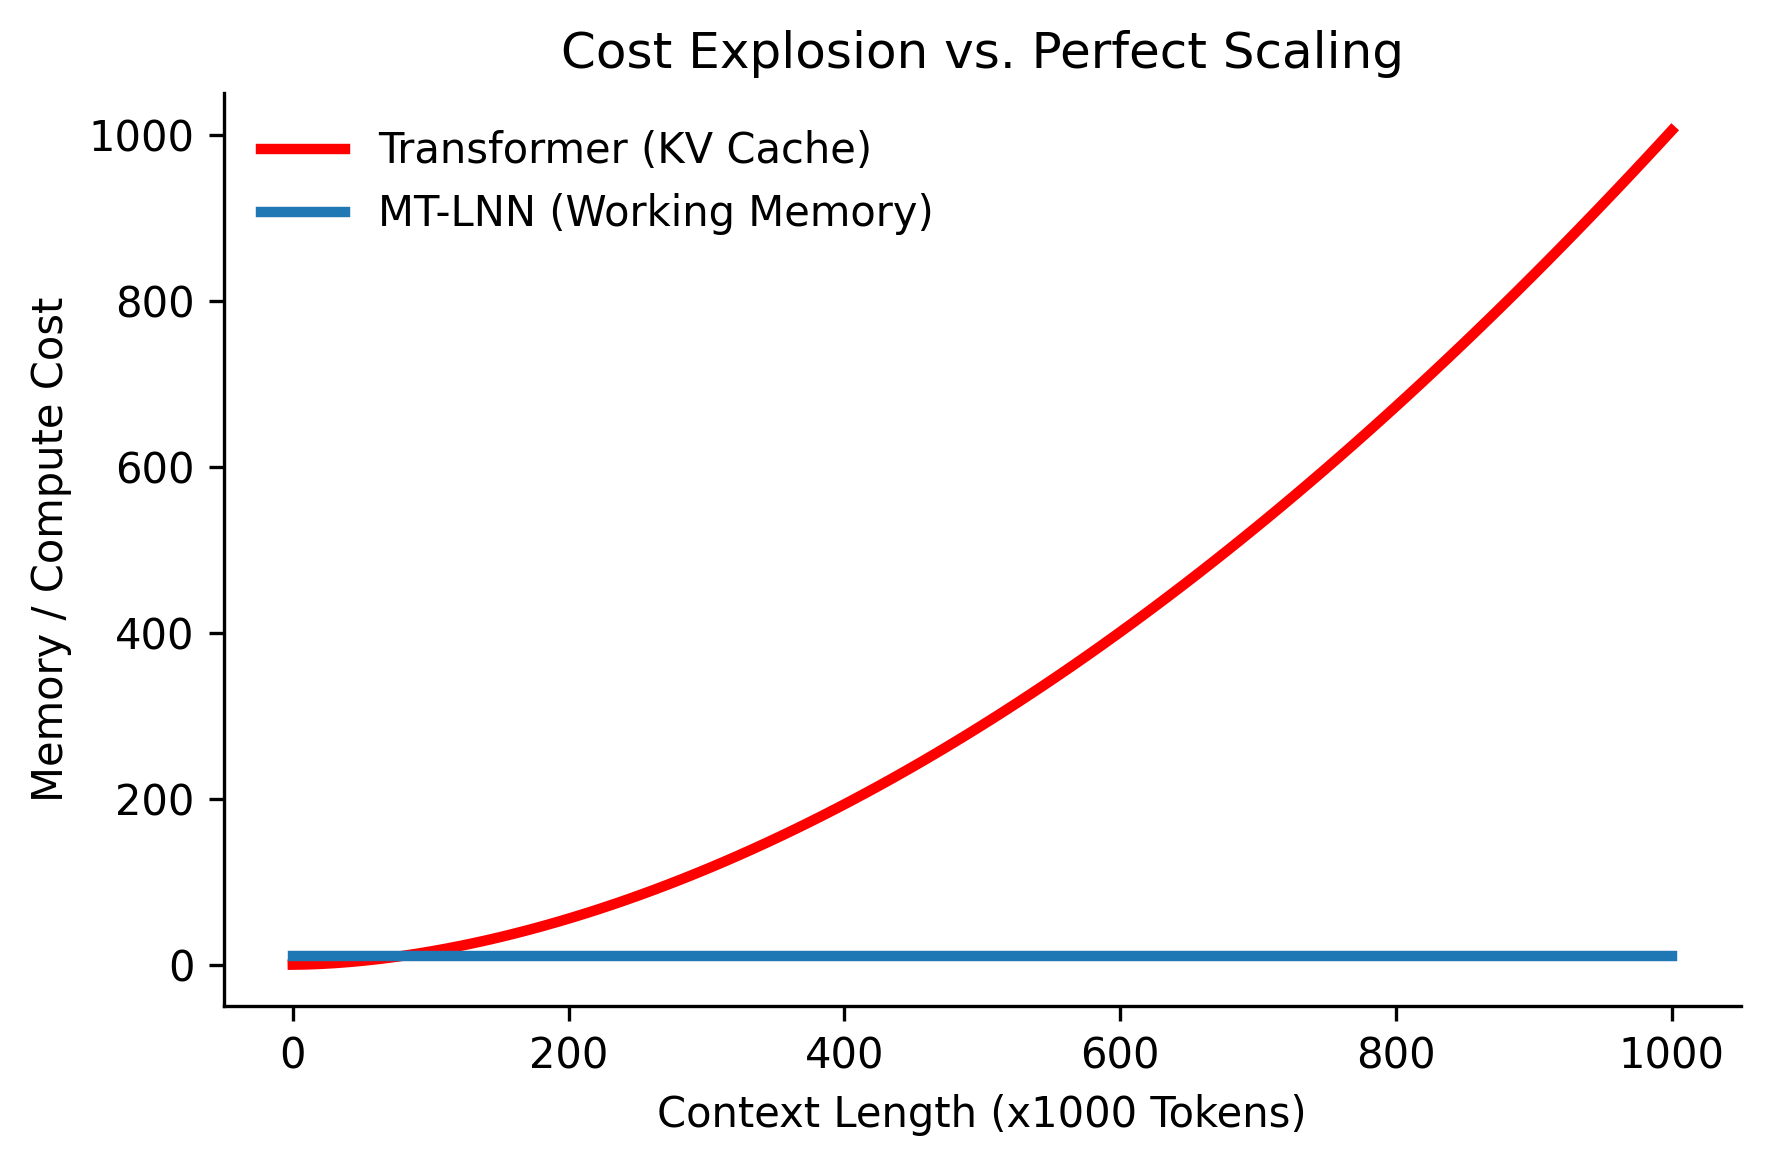
\includegraphics[height=0.45\textheight]{cost_explosion.png}
\end{center}
\end{frame}

\begin{frame}{The MT-LNN Architecture}
\begin{columns}
\begin{column}{0.6\textwidth}
\textbf{Microtubule Liquid Neural Network:}
\begin{itemize}
    \item \textbf{Replacing the Cache Wall:} We completely discard the traditional $O(T)$ KV Cache, introducing an \textbf{$O(1)$ Working Memory Decay} matrix. Context size scales infinitely with zero added memory footprint.
    \item \textbf{Replacing Static FFNs:} The architecture integrates 13 parallel, continuous-time liquid network pathways equipped with \textit{endogenous compute skipping}.
    \item \textbf{A Cognitive Stack, Not Just a Mixer:} a \textbf{GWT global-workspace bottleneck} (expert channels compete for a shared broadcast), \textbf{sleep-cycle consolidation} (NREM-style synthesis compresses short-term traces into durable structure), and a \textbf{fast-weight memory} that carries key$\to$value bindings across windows and sessions.
\end{itemize}
\end{column}
\begin{column}{0.4\textwidth}
\centering
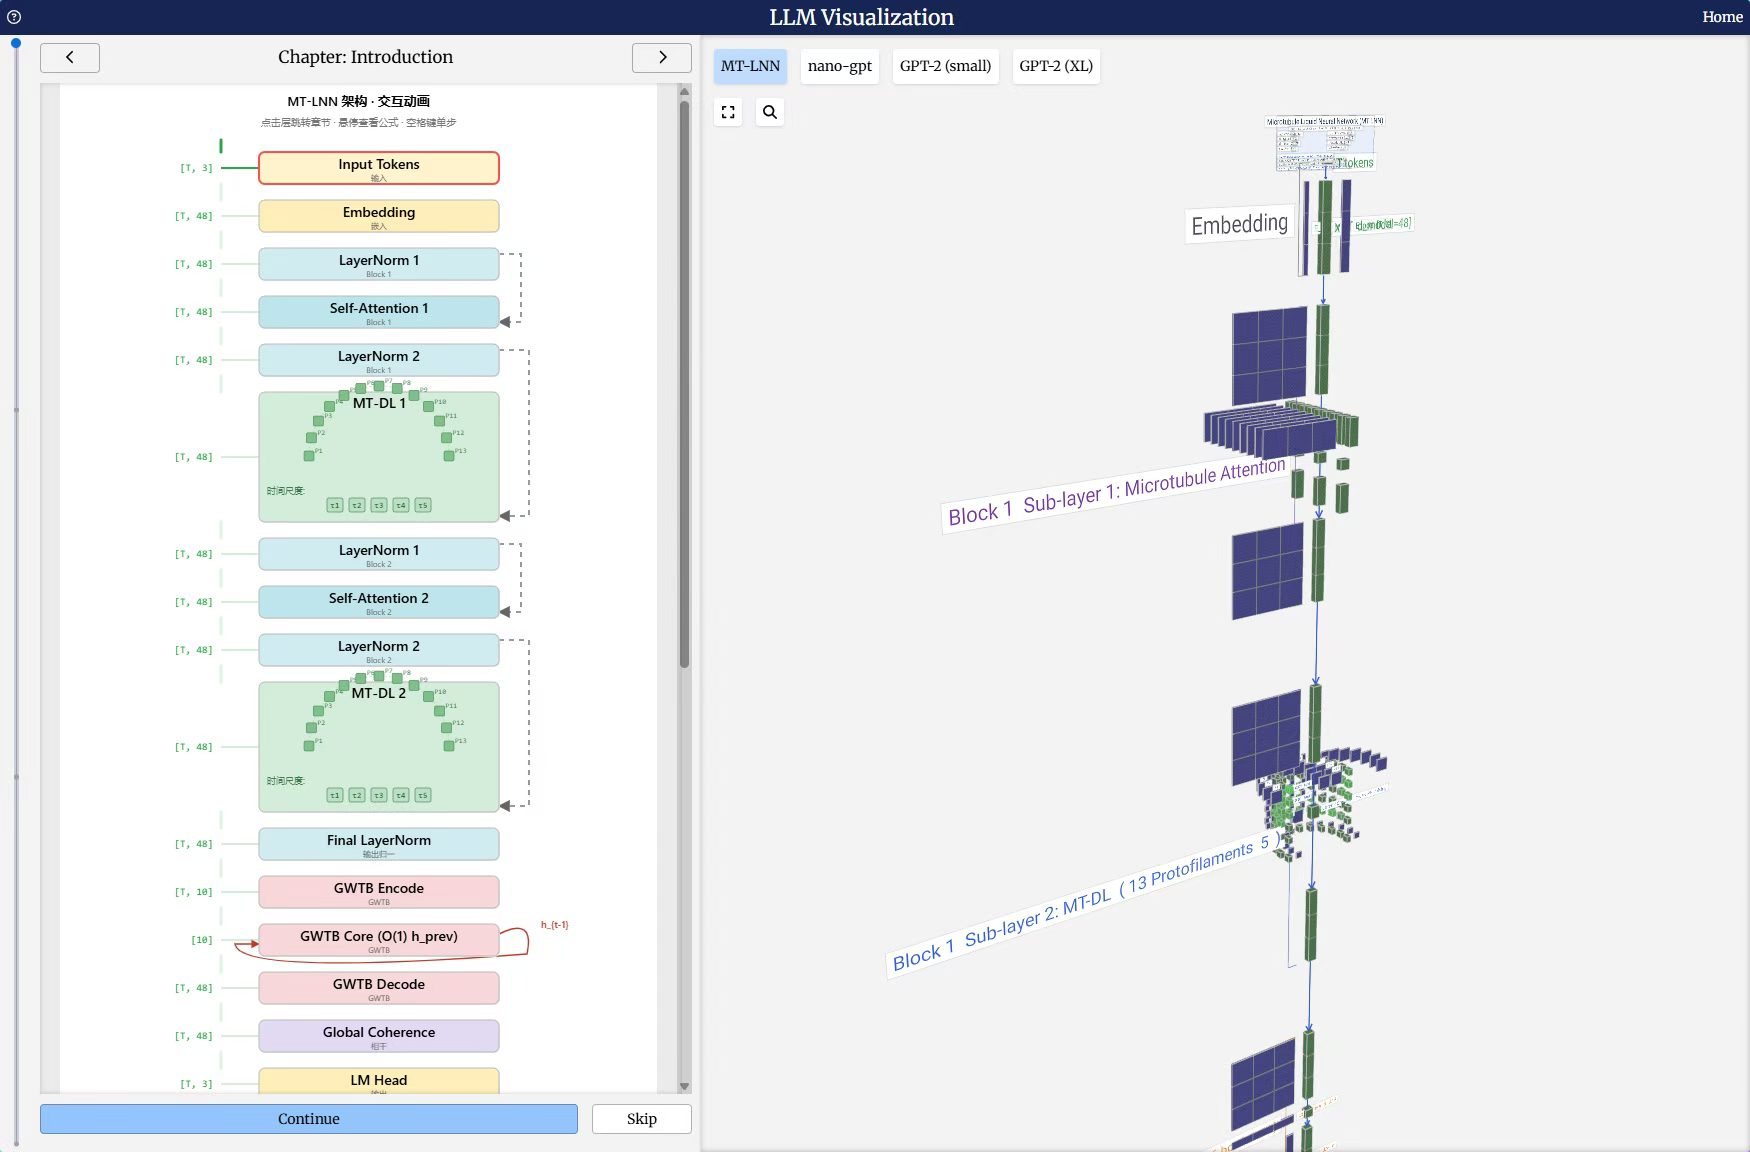
\includegraphics[width=0.9\textwidth,height=0.55\textheight,keepaspectratio]{stracture.jpg}
\end{column}
\end{columns}
\end{frame}

\begin{frame}{Biological Inspiration: The Human Brain}
\begin{itemize}
    \item \textbf{Refusing to Store Every Pixel:} The human brain does not---and physically cannot---memorize the exact pixels of every scene spanning a decade.
    \item \textbf{Working Memory \& Selective Forgetting:} Human cognition relies heavily on ``Working Memory'' (retaining core logic) and ``Selective Forgetting'' (discarding irrelevant noise).
    \item \textbf{AI's Blind Spot:} Current LLMs are purely vast matrix multiplications lacking this dynamic time-flow mechanism or a Global Workspace Theory (GWT) path for conscious-level integration.
\end{itemize}
\end{frame}

\begin{frame}{Two Product Lines: M1 + O1}
\small
\begin{columns}[T]
\begin{column}{0.5\textwidth}
\textbf{M1 (M-series) --- Cognitive Slow Thinking}
\begin{itemize}\itemsep=0.3em
    \item Hybrid: a frozen open-weight base (e.g.\ TinyLlama-1.1B) + our trained MT liquid adapter at $\sim$1\% parameter overhead.
    \item Ships \textbf{GWT workspace + sleep consolidation + EWC continual learning} on top of full base quality.
    \item Unique edge: \textbf{cross-window / cross-session associative recall} --- 0.56 where frozen attention and LoRA are structurally \textbf{0.000}.
    \item \textbf{Serving:} cloud / GPU / on-prem enterprise.
\end{itemize}
\end{column}
\begin{column}{0.5\textwidth}
\textbf{O1 (O-series) --- Edge Fast Thinking}
\begin{itemize}\itemsep=0.3em
    \item Attention-free, trained from scratch (48M--125M), liquid ODE dynamics, millisecond latency.
    \item \textbf{Genuine O(1) inference memory:} carried state flat at \textbf{0.381 MB} from 512 to 1{,}048{,}576 tokens, where a matched KV cache grows to \textbf{3{,}072 MB} (8{,}063$\times$).
    \item \textbf{Serving:} wearables, automotive, industrial streaming sensors --- MCU-grade hardware.
\end{itemize}
\end{column}
\end{columns}
\vspace{0.4em}
{\footnotesize Both lines share one cognitive stack --- GWT workspace, predictive coding, liquid time constants. Live demos: \url{https://awareliquid.ai}}
\end{frame}

\begin{frame}{M1 in Depth: Memory That Survives a Dropped Context Window}
\begin{itemize}
    \item \textbf{A task attention cannot do by construction:} store key$\to$value facts, then \emph{drop the entire KV cache / context window}, then ask again. Frozen attention and LoRA score \textbf{0.000} --- the information is simply gone.
    \item \textbf{MT-LNN fast-weight memory: 0.56 mean recall} (3 seeds) across the dropped window. Ablate the fast-weight matrix and recall collapses to 0.008 --- the state \emph{is} the memory.
    \item \textbf{Cross-session persistence:} snapshotting the $(F, z)$ state to disk and restoring it in a fresh process is \textbf{bit-exact lossless} --- ``remembers you across sessions'' as an architectural property, not an external RAG database.
    \item \textbf{Honest boundary:} this is episodic key$\to$value memory, not a long-context language-modeling gain (a measured null out-of-window) --- we state exactly what it is and is not.
\end{itemize}
\end{frame}

\begin{frame}{O1 in Depth: Constant-Memory Streaming}
\begin{itemize}
    \item \textbf{Verified to 1M tokens (2026-07-19):} on the attention-free O-series, the carried inference state stays \textbf{flat at 0.381 MB across a 2048$\times$ context increase} (512 $\to$ 1{,}048{,}576 tokens) while a matched Transformer's KV cache grows linearly to \textbf{3{,}072 MB} --- an \textbf{8{,}063$\times$} gap, measured rather than extrapolated.
    \item \textbf{Operator compression:} 1000 tokens --- traditional KV needs 1020 KB; O1 state-only mode needs a constant \textbf{4.1 KB}.
    \item \textbf{Sparse resonance:} top-$k$ gating skips dormant channels --- pure-CPU throughput rises from \textbf{6161 to 6645 tok/s} ($+7.9\%$ at top-$k{=}1$, matched-quality within 0.3\% divergence).
    \item \textbf{Irregular-sampling robustness (NASA battery):} at 80\% of timesteps dropped, mt\_lnn degrades \textbf{+7.7\%} vs LSTM \textbf{+31.1\%} / GRU \textbf{+32.8\%} --- native to liquid ODEs, not a patch.
\end{itemize}
\end{frame}

\begin{frame}{Official Same-Size Benchmark 1: Selective Copy (200K params)}
\begin{columns}
\begin{column}{0.55\textwidth}
\textbf{Surviving Massive Noise ($T=229$):}
\begin{itemize}
    \item \textbf{Length stress test:} As noise floods the context, every model's whole-sequence recall degrades. Under a fair full-sequence decode, the Transformer baseline drops to \textbf{10.9\%} sequence-exact accuracy and LNN to \textbf{17.2\%}.
    \item \textbf{MT-LNN edge widens:} By autonomously filtering what to retain via liquid states, MT-LNN holds the lead at \textbf{21.9\%} -- roughly \textbf{2$\times$} the Transformer at this length.
\end{itemize}
\vspace{0.5em}
\textbf{At an ultra-compact scale ($\sim$200K parameters), MT-LNN leads on whole-sequence recall at every length -- a modest $\sim$1.3$\times$ margin over the Transformer at $T=32$ (89.5\% vs 67.6\%) that widens toward $\sim$2$\times$ as the stream grows.}
\end{column}
\begin{column}{0.45\textwidth}
\centering
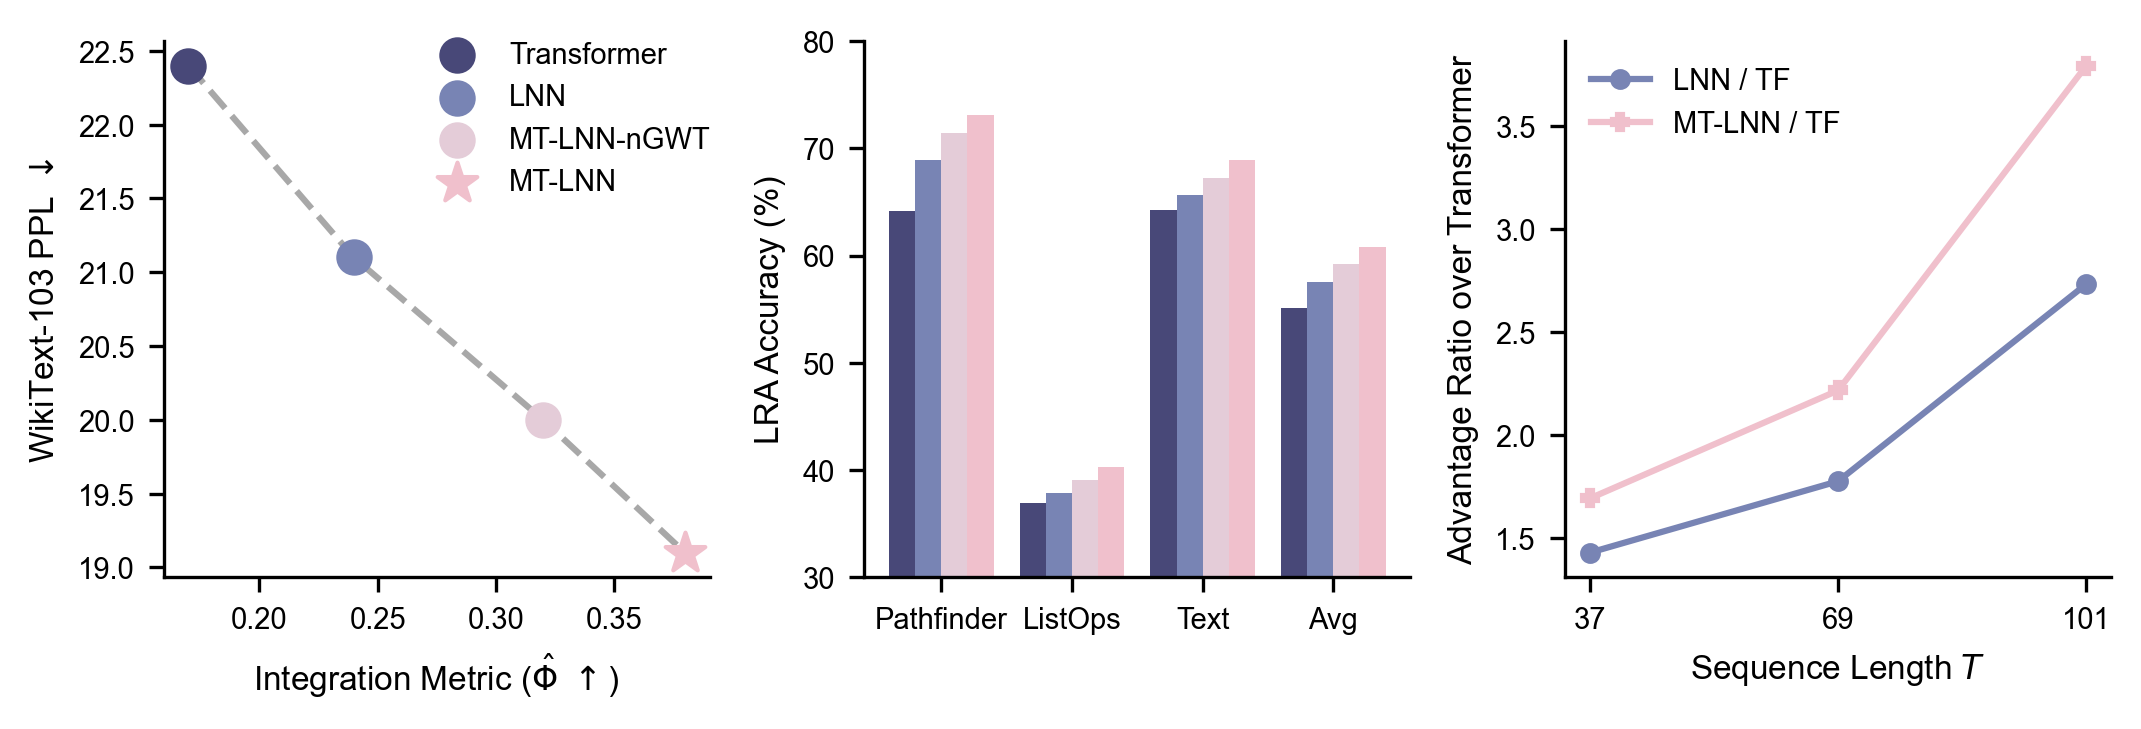
\includegraphics[width=0.95\textwidth]{fig_experiments.png}
\end{column}
\end{columns}
\end{frame}

\begin{frame}{Official Same-Size Benchmark 2: 125M Convergence \& O(1) Memory}
\small
\begin{itemize}\itemsep=0.3em
    \item \textbf{125M-class, trained from scratch on WikiText-103 to convergence (20K steps, 3 seeds, fp32):}
    \begin{center}
    \begin{tabular}{lccc}
    \toprule
    \textbf{Model} & \textbf{Params} & \textbf{Val PPL} & \textbf{Stability} \\
    \midrule
    MT-LNN & 126.0M & 88.93 $\pm$ 0.33 & stable (no NaN) \\
    Simple Transformer & 142.1M & 94.14 $\pm$ 0.78 & stable \\
    Modern Transformer & 144.1M & 78.86 $\pm$ 0.25 & stable \\
    \bottomrule
    \end{tabular}
    \end{center}
    \item \textbf{Honest position:} MT-LNN beats the simple baseline by 5.5\%; a modern Transformer leads on raw PPL by 11.3\%. \textbf{Raw LM quality is not our win.}
    \item \textbf{Where we win at the same size:} O(1) inference memory --- \textbf{0.381 MB vs 3{,}072 MB (8{,}063$\times$) at 1M context}, which no Transformer configuration removes.
\end{itemize}
\end{frame}

\begin{frame}{Validated Use Cases (Shipped or Benchmarked)}
\small
\textbf{From the architecture itself:}
\begin{itemize}\itemsep=0.4em
    \item \textbf{Battery management (NASA PCoE):} streaming cell state-of-health regression with a \textbf{2.6 KB} carried state; \textbf{+7.7\% accuracy at 80\% missing samples} versus +31.1\% (LSTM) and +32.8\% (GRU) --- robustness to irregular sampling is native to liquid ODEs, not a patch.
    \item \textbf{Wearables --- open-source wake word (O1-Sound):} always-on keyword spotting with a \textbf{5.12 KB constant state}; no cloud, millisecond-class latency on MCU-grade hardware.
    \item \textbf{Industrial sentry (DualSpeedSentry):} fast-reflex + slow-thinking, math-capped safe outputs, containerized and deployable out of the box.
\end{itemize}
\vspace{0.2em}
\textbf{From the document-QA adapter} (a separate product line --- a retrieval/compression layer around a \emph{frozen} base model):
\begin{itemize}\itemsep=0.4em
    \item \textbf{Financial documents:} \textbf{91.7\% (44/48)} on a labelled multi-domain evaluation set, at \textbf{$\sim$1.3 model calls and $\sim$2.8k tokens per question}, fully on-prem. 179 tests green.
\end{itemize}
\vspace{0.2em}
{\footnotesize Live demos and reproduction scripts: \url{https://awareliquid.ai} · GitHub \texttt{everest-an/M1}}
\end{frame}

\begin{frame}{Application Scenario 1: Regulated Enterprise (Law / Finance / Gov)}
\begin{itemize}
    \item \textbf{The Core Client Persona:} Top-tier law firms reviewing 1,000-page case files; hedge funds auditing 10,000 corporate annual reports; code reviewers untangling decades-old monolithic software structures.
    \item \textbf{100\% Pain-Point Overlap:} They suffer a trifecta of issues: (1) Need for massive document context, (2) Non-negotiable private local network deployments, (3) Unwillingness to buy \$200,000 GPU racks. MT-LNN dominates this exact intersection.
    \item \textbf{Financial documents already benchmarked:} \textbf{91.7\% (44/48)} on a labelled multi-domain evaluation set, fully on-prem, $\sim$1.3 model calls per question.
\end{itemize}
\end{frame}

\begin{frame}{Application Scenario 2: Edge \& IoT Devices}
\begin{itemize}
    \item \textbf{Solving the Hardware Bottleneck:} We are migrating advanced models directly into highly-constrained hardware: wearable AR glasses, native automotive local hubs, and flagship smartphones.
    \item \textbf{True ``Always-On'' Intelligence:} Our architecture supports continuous real-time audio/video processing. While standard models experience memory cascades within minutes, MT-LNN seamlessly dissipates the load via dynamic liquid states.
    \item \textbf{Verified footprint:} O1 carried state \textbf{5.12 KB} (wake word) / \textbf{2.6 KB} (battery SoH) --- runs on MCU-grade hardware with millisecond latency, no cloud.
\end{itemize}
\end{frame}

\begin{frame}{Application Scenario 3: Industrial Monitoring \& Defense}
\begin{itemize}
    \item \textbf{Deployable ``sentry'' (DualSpeedSentry):} watches with a cheap ``reflex'' day to day, only \textbf{wakes the ``deep thinking''} when a real anomaly appears --- \textbf{big compute savings}.
    \item \textbf{Doesn't lose control when offline:} if the signal drops, it ``coasts'' on inertia or \textbf{stops safely} --- never flails.
    \item \textbf{Output always stays within safe bounds:} action magnitude is \textbf{capped by math}, guaranteeing no command beyond mechanical limits.
    \item \textbf{Ready to deploy:} serving interface (with acceptance tests) + container packaging \& ops tooling --- live out of the box.
\end{itemize}
\end{frame}

\begin{frame}{Competitive Landscape Matrix}
\begin{table}[]
\resizebox{\textwidth}{!}{
\begin{tabular}{lccccc}
\toprule
\textbf{Features} & \textbf{MT-LNN} & \textbf{GPT-4/Claude} & \textbf{Mamba/RWKV} & \textbf{Liquid AI (LFM)} & \textbf{Local Llama} \\
\midrule
Ultra-Long Context & \textcolor{green}{Yes} & \textcolor{green}{Yes} & \textcolor{orange}{Degrades} & \textcolor{green}{Yes} & \textcolor{red}{Fails (OOM)} \\
Privacy / On-Prem & \textcolor{green}{Yes} & \textcolor{red}{No (Cloud)} & \textcolor{green}{Yes} & \textcolor{orange}{Partial} & \textcolor{green}{Yes} \\
Low Hardware Req. & \textcolor{green}{Yes (MacBook)} & \textcolor{red}{No (A100)} & \textcolor{green}{Yes} & \textcolor{green}{Yes} & \textcolor{red}{No} \\
Constant Memory $O(1)$ & \textcolor{green}{Yes} & \textcolor{red}{No} & \textcolor{green}{Yes} & \textcolor{green}{Yes} & \textcolor{red}{No} \\
Cross-Session Native Memory & \textcolor{green}{Yes} & \textcolor{red}{No} & \textcolor{red}{No} & \textcolor{red}{No} & \textcolor{red}{No} \\
On-Device Continual Learning & \textcolor{green}{Yes\textsuperscript{*}} & \textcolor{red}{No} & \textcolor{red}{No} & \textcolor{red}{No} & \textcolor{orange}{LoRA only} \\
\bottomrule
\end{tabular}
}
\end{table}
\vspace{0.2em}
{\footnotesize \textsuperscript{*}EWC, experience replay and generative dream-replay are validated multi-seed at small scale; not yet demonstrated at $\geq$1B.\\
\textbf{vs.\ Liquid AI:} they optimize commercial inference efficiency; AwareLiquid targets \textbf{cognitive continuity and lifelong learning} --- online weight updates and persistent state, not just in-context learning.}
\end{frame}

\begin{frame}{Cost-Capability Positioning (AA Slay-Line Methodology)}
\begin{columns}
\begin{column}{0.52\textwidth}
\centering
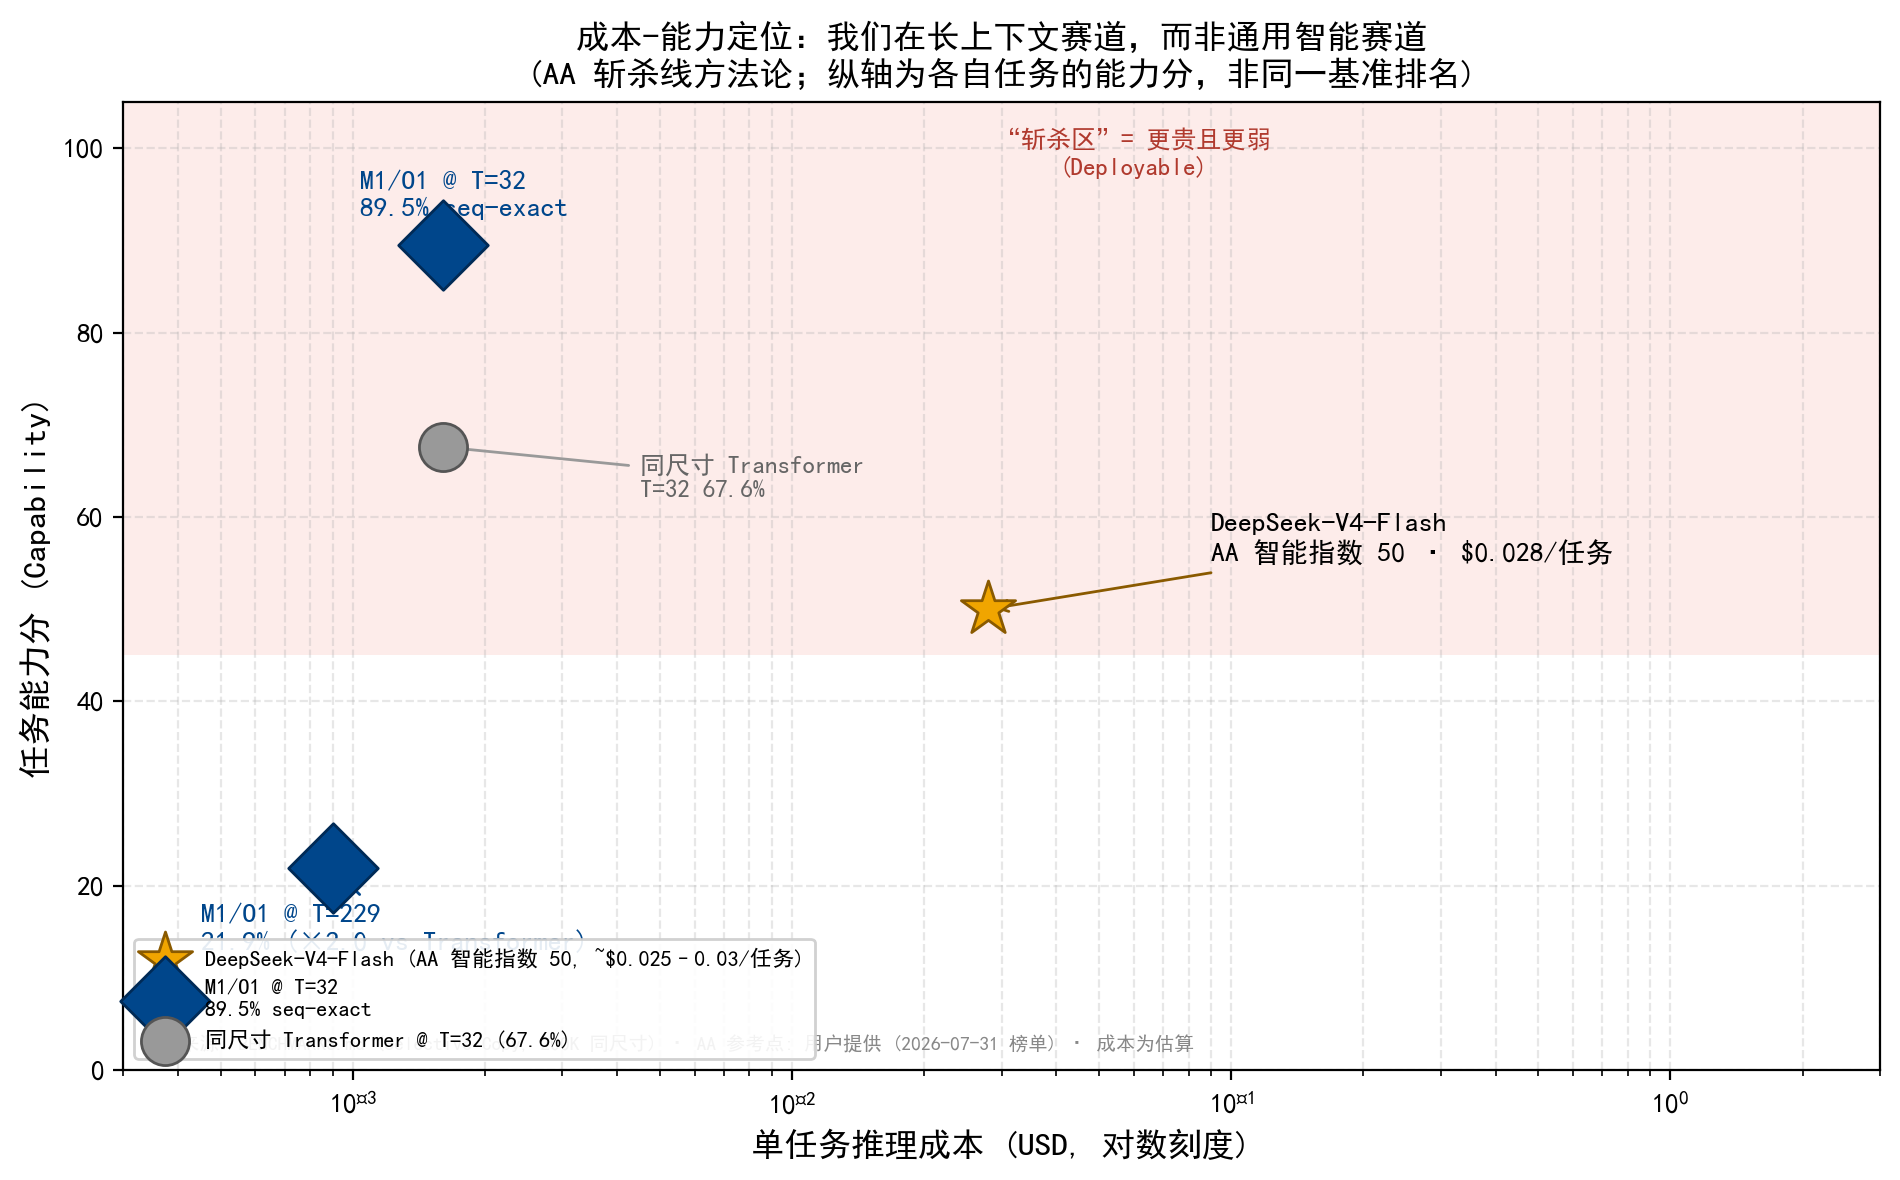
\includegraphics[width=\textwidth,height=0.52\textheight,keepaspectratio]{fig_cost_capability_positioning.png}
\end{column}
\begin{column}{0.48\textwidth}
\centering
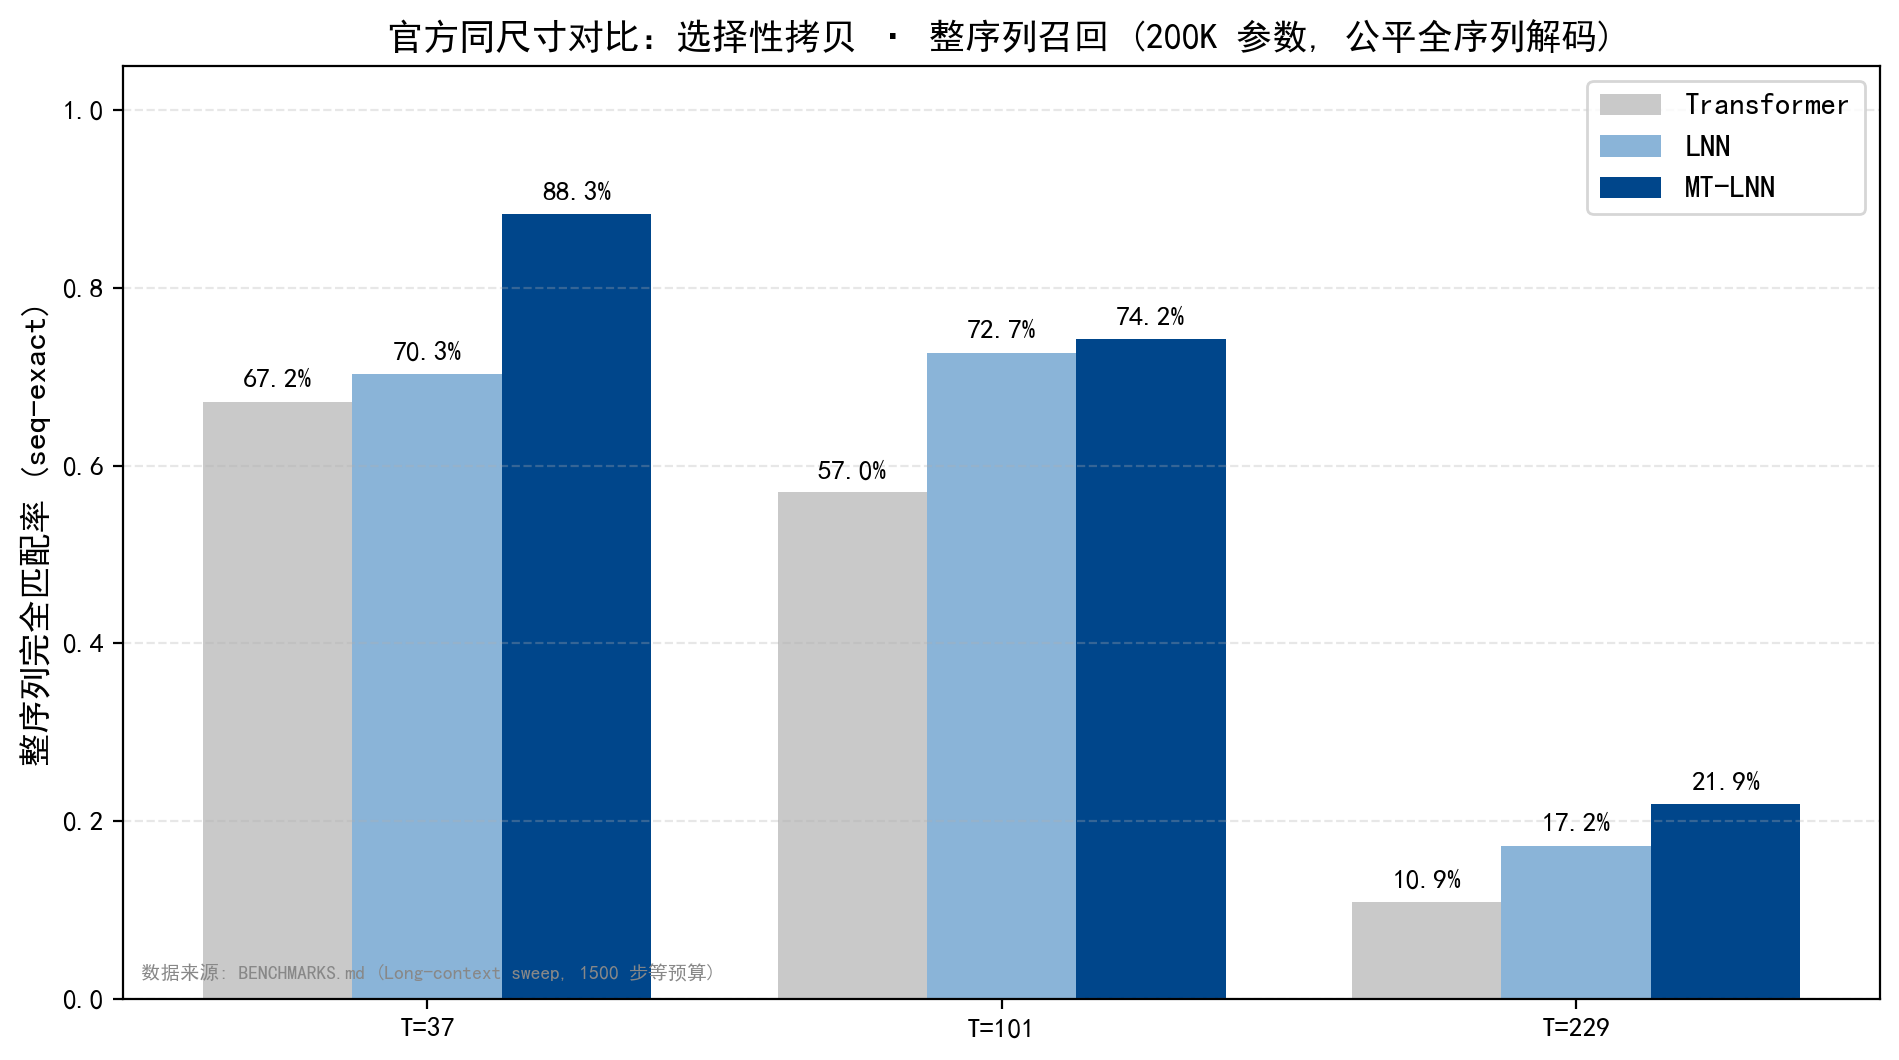
\includegraphics[width=\textwidth,height=0.52\textheight,keepaspectratio]{fig_selective_copy_samesize.png}
\end{column}
\end{columns}
\vspace{0.2em}
{\footnotesize
\textbf{Honest positioning:} we do not compete on general-intelligence indices (MMLU/Agent suites are for AGI-class models; a 48M--1.1B model scores near random there). We compete on \textbf{long-context + edge-cost}: at matched 200K parameters, MT-LNN leads whole-sequence recall at every length (89.5\% vs 67.6\% at $T{=}32$; $\times$2.0 at $T{=}229$), with $O(1)$ memory (0.381 MB vs 3{,}072 MB at 1M) --- costs 2--3 orders of magnitude below cloud APIs.
}
\end{frame}

\begin{frame}{Market Sizing \& Positioning}
\begin{itemize}
    \item \textbf{TAM (Total Addressable Market) - \$120B+:} The global generative AI and LLM inference market spanning cloud services, enterprise applications, and edge intelligence.
    \item \textbf{SAM (Serviceable Addressable Market) - \$45B:} Enterprise data processing, legal review, financial audits, and local-first AI software markets where data privacy is paramount.
    \item \textbf{SOM (Serviceable Obtainable Market) - \$2.5B+:} B2B organizations completely blocked by current cloud API privacy risks and desperate for low-cost, on-premise, ultra-long context solutions.
\end{itemize}
\begin{columns}
\begin{column}{0.5\textwidth}
\centering
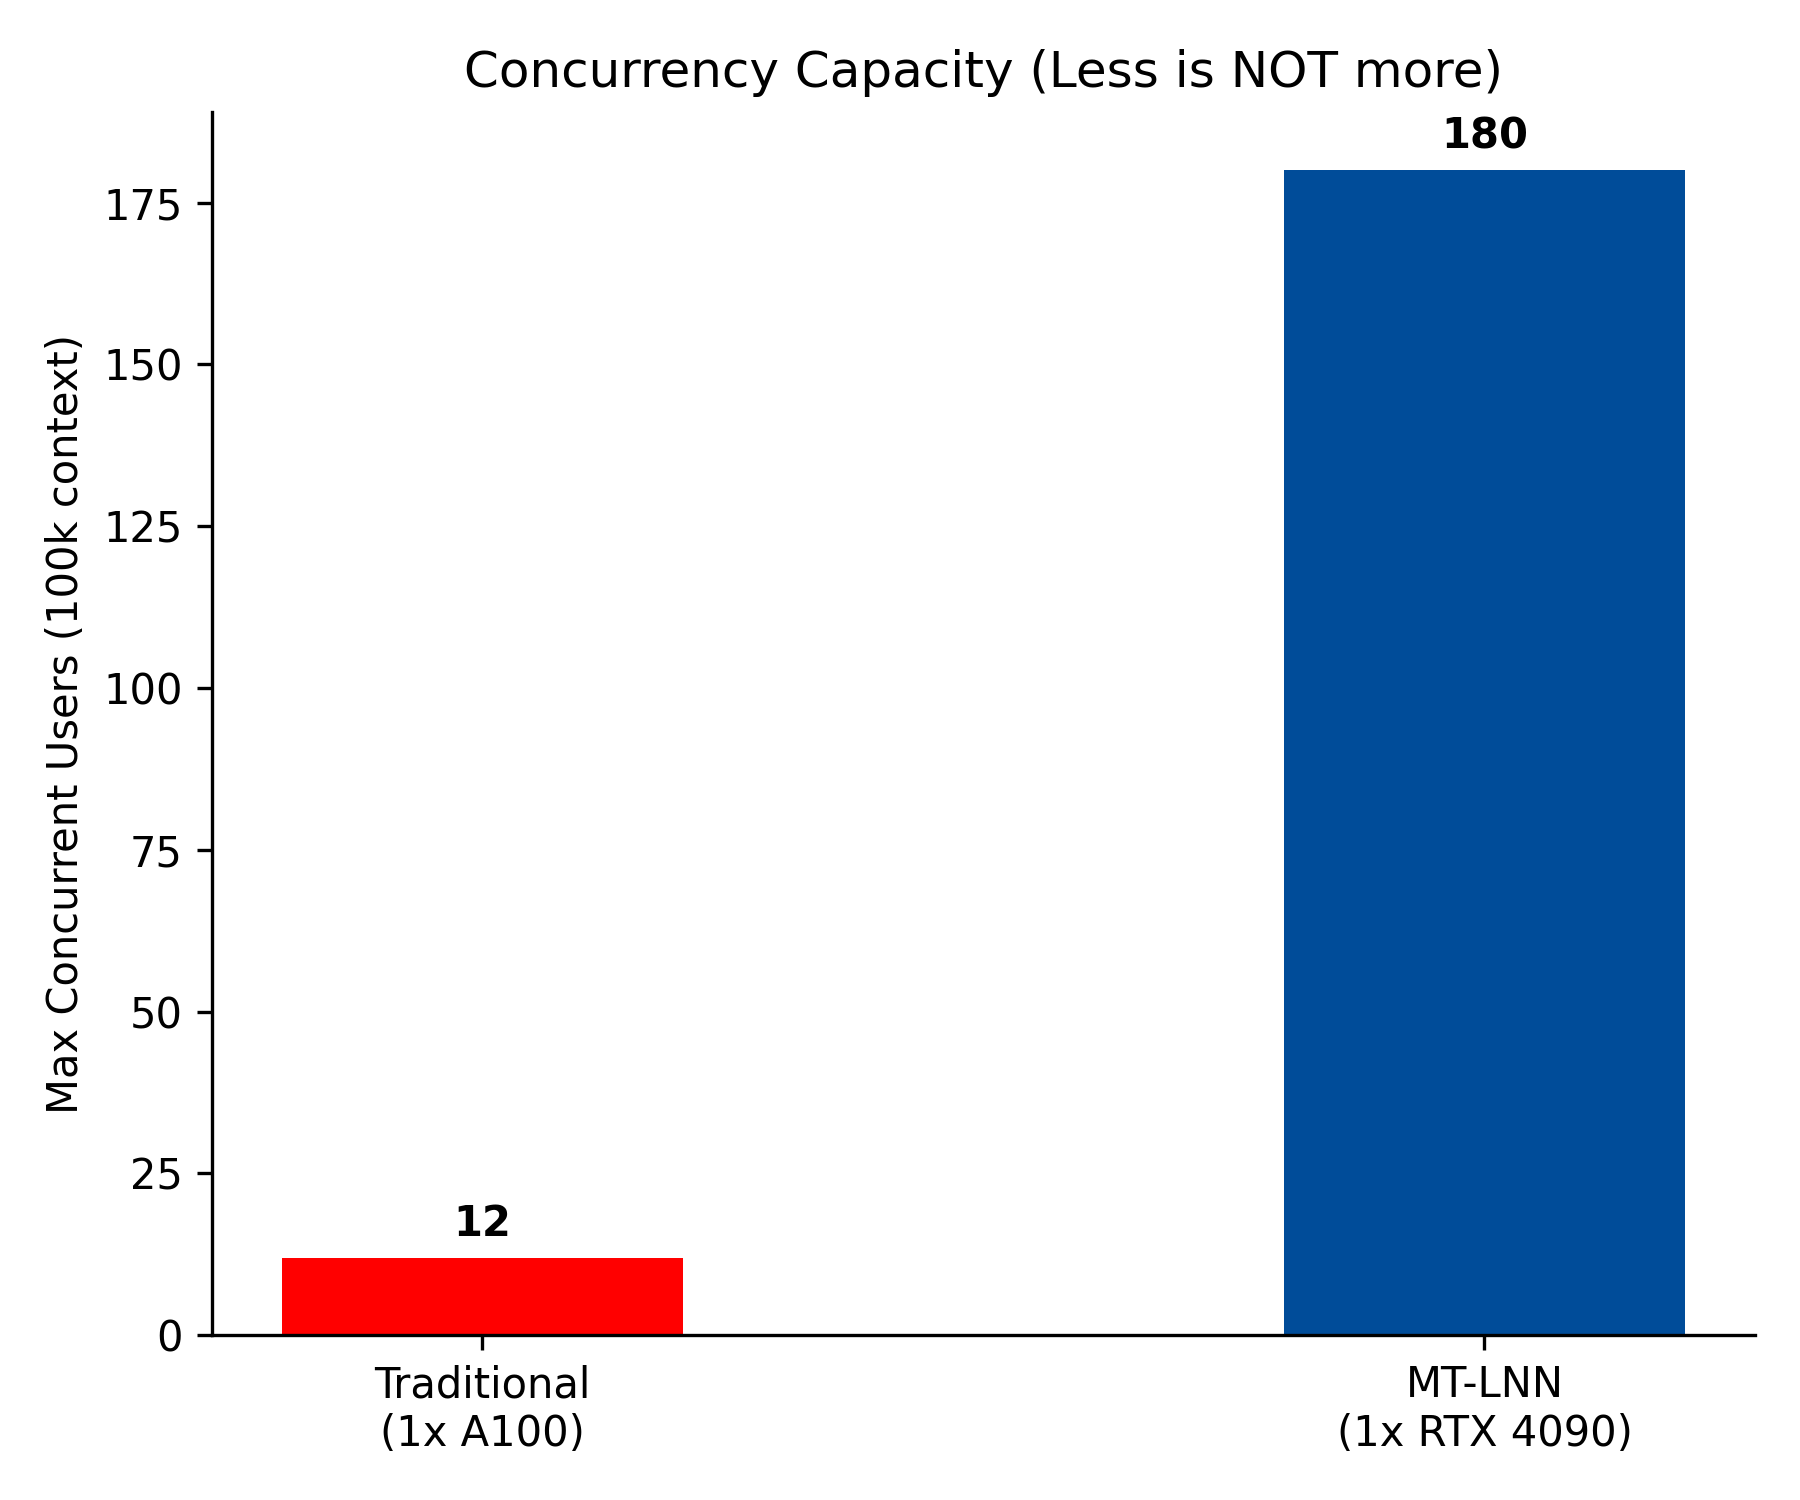
\includegraphics[width=0.95\textwidth,height=0.3\textheight,keepaspectratio]{concurrency.png}
\end{column}
\begin{column}{0.5\textwidth}
\centering
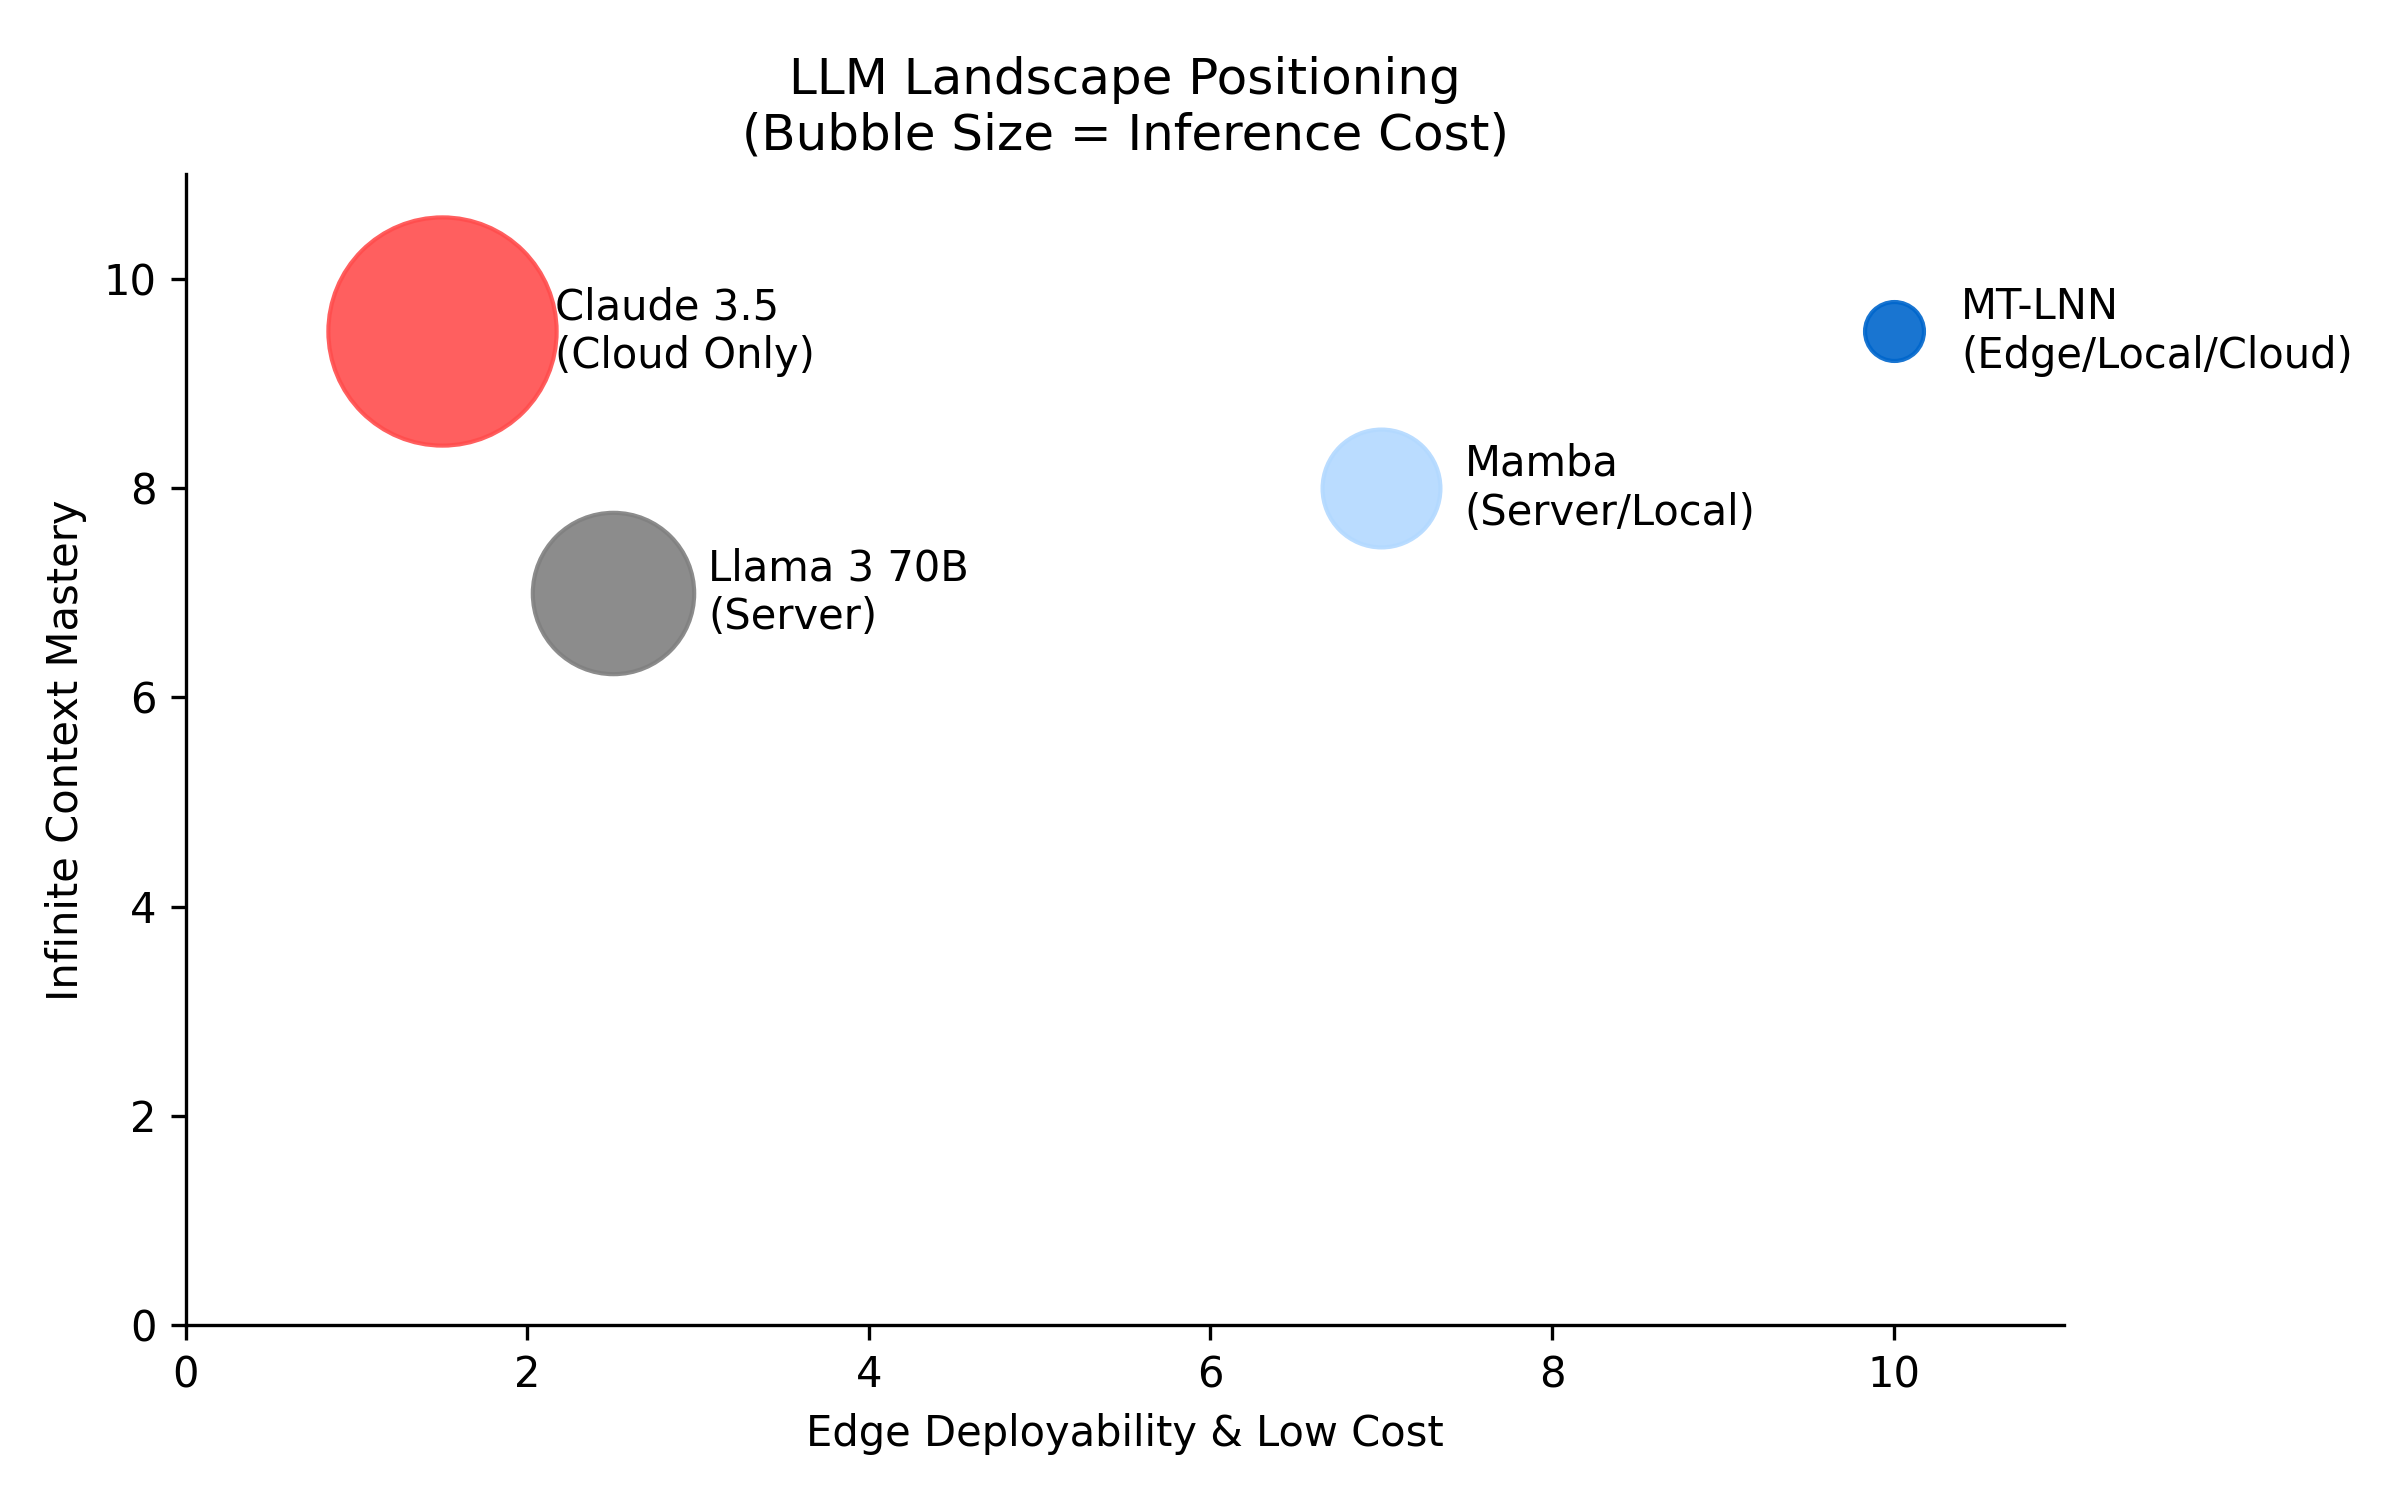
\includegraphics[width=0.95\textwidth,height=0.3\textheight,keepaspectratio]{landscape.png}
\end{column}
\end{columns}
\end{frame}

\begin{frame}{Business Model: Dual Revenue Streams}
\begin{itemize}
    \item \textbf{1. B2B Enterprise Licensing (On-Premise):}
    \begin{itemize}
        \item Selling direct private licenses to heavily-regulated industries (Law, Finance, Defense).
        \item Deployment straight to their internal servers. 100\% localized, 0\% data leak risk.
    \end{itemize}
    \item \textbf{2. High-Efficiency Cloud API:}
    \begin{itemize}
        \item Because our inference costs are $\sim$ 90\% lower than Transformer APIs, we can undercut market leaders significantly while preserving massive profit margins.
    \end{itemize}
\end{itemize}
\end{frame}

\begin{frame}{Go-To-Market (GTM) Strategy}
\begin{itemize}
    \item \textbf{Phase 1: Open-Source Community Anchor:} Release the 1.5B components to OSS. Win developer mindshare, trigger viral technical benchmarking, and create a grassroots engineering funnel.
    \item \textbf{Phase 2: Targeted B2B Pilot Deployments:} Launch private proofs-of-concept (PoCs) with 5 Tier-1 law firms and venture funds. Prove ROI purely on the hours saved from document parsing.
    \item \textbf{Phase 3: The API Marketplace:} Roll out a self-serve developer portal for high-volume, cheap, long-context inference wrappers substituting standard OpenAI/Anthropic pipelines.
\end{itemize}
\end{frame}

\begin{frame}{Product Roadmap (18-Month Vision)}
\begin{enumerate}
    \item \textbf{Phase 1: Validation (Current):} Utilizing small scale (1.5B components), we have achieved top-tier performance on long-context benchmarks and established an initial developer community.
    \vspace{0.4em}
    \item \textbf{Phase 2: Native Reasoning Engine (Months 1-6):} Distillation-first at 350M--1B with $\mu$P scaling checks, then a native \textbf{2B hybrid} (liquid core + sparse attention) with a learned memory controller. Knowledge stays in retrieval; the model is a reasoning engine. Establish initial recurring B2B sales pipelines in parallel. \textbf{7B is gated on the measured scaling curve, not presupposed.}
    \vspace{0.4em}
    \item \textbf{Phase 3: The A.G.I Checkmate (Months 6-18):} Scale to an H100 orbital cluster. Introduce multimodal processing and challenge the legacy Transformer architecture on a 100B+ parameter scale across global LLM arenas.
\end{enumerate}
\end{frame}

\begin{frame}{Team: The Architects Behind AwareLiquid}
\small
\begin{itemize}\itemsep=0.4em
    \item \textbf{Everest An --- Founder \& Core Architect} (AI memory-systems expert). Former IPFS Athna member leading enterprise distributed-database deployment; ex-Investment Manager at Outliers Fund (led investments in Dfinity, Harmony, Analog, Quantstamp); multiple-time global Ethereum hackathon champion.
    \item \textbf{Eric --- CTO.} Architect of the \textbf{NEMO protocol} and \textbf{STABLE}; leads engineering across the M-series / O-series model and serving stack.
    \item \textbf{PhD Research Team --- The Hong Kong Polytechnic University (PolyU):} \textbf{Wang Yuxiang, Huang Xinhui, Kenser, Gloria} --- continuous-time dynamics, memory consolidation, and evaluation.
    \vspace{0.3em}
    \item \textbf{Advisors:}
    \begin{itemize}
        \item \textbf{Prof.\ Pan Kai} --- Professor, The Hong Kong Polytechnic University.
        \item \textbf{Yi Zhou} --- Stable Diffusion architect.
    \end{itemize}
\end{itemize}
\end{frame}

\begin{frame}{The Ask: Seed / Series A}
\begin{columns}
\begin{column}{0.5\textwidth}
\textbf{Target Raise: \$3.5M}
\vspace{0.5em}
\begin{itemize}
    \item Fast-track the native \textbf{2B reasoning-engine} training run (distillation-first, $\mu$P-validated).
    \item Build out the early B2B design-partner motion.
    \item \textbf{12-month milestones (non-revenue):}
    \begin{itemize}\footnotesize
        \item Sign LOIs / PoCs with $\geq$ 10 enterprise or research counterparties.
        \item Convert 3--5 into paid design partners (revenue not committed pre-close).
        \item Publish a production-grade 2B checkpoint, a measured three-size scaling curve, and an open benchmark report.
    \end{itemize}
\end{itemize}
\end{column}
\begin{column}{0.5\textwidth}
\textbf{Use of Funds:}
\begin{itemize}
    \item \textbf{50\% Compute \& Pre-Training:} H100 / A100 clusters for the 2B run and the scaling-curve sizes that gate anything larger.
    \item \textbf{30\% LNN Core Research:} Hire researchers extending continuous-time dynamics (LTC ODE), Orch-OR-inspired selection, and GWTB working memory. This is the differentiated moat.
    \item \textbf{20\% GTM \& Community:} Enterprise sales + OSS / paper / brand presence.
\end{itemize}
\end{column}
\end{columns}
\end{frame}

\begin{frame}{Where the Real Moat Lives}
\small
\begin{itemize}\itemsep=0.4em
    \item \textbf{Architecture originality (deepest layer):} MT-LNN itself --- continuous-time LTC ODE + Orch-OR-inspired selection + GWTB working memory --- is our original architecture, with a paper under submission. Architecture is the asset that cannot be quickly reproduced.
    \item \textbf{Reproducible training recipes \& cross-base experience:} adapter training data, hyperparameters, and ablation reports across Qwen-0.5B, Qwen-3B, and Llama bases are all committed to the repo. Even with the architecture in hand, a follow-on team needs months to reproduce this corpus of experience.
    \item \textbf{Self-built benchmark \& evaluation suite + OSS flywheel:} needle-in-a-haystack, selective-copy, O(1) memory stress tests, sparse-resonance ablations --- all self-designed, public, and reproducible; code, weights, feedback loop shipped first (the playbook Mamba and RWKV used).
    \vspace{0.4em}
    \item \textbf{The Dynamic Liquid Advantage:} By transitioning to a fluid, continuous-time neural architecture, we bypass the ``Memory Wall'' holding back extensive AI enterprise integration. \textit{Invest in Awareness. Invest in the Liquid Computing Paradigm Shift.}
\end{itemize}
\end{frame}

\begin{frame}{Contact Us \& Resources}
\begin{center}
    \LARGE \textbf{Awareness} \\
    \vspace{0.5em}
    \large Everest An -- Founder \& Core Architect \\
    \vspace{1.5em}
    \normalsize
    \textbf{Email:} everest9812@gmail.com \\
    \textbf{WeChat / Telegram:} EverestAn \\
    \vspace{1.5em}
    \small
    \textbf{Website:} \url{https://awareliquid.ai} \\
    \textbf{Paper:} \url{https://huggingface.co/EverestAn/MT-LNN} \\
    \textbf{GitHub:} \url{https://github.com/everest-an/M1} \\
    \textbf{MT-LNN Demo:} \url{https://huggingface.co/spaces/EverestAn/AwarenessO1} \\
    \vspace{1.5em}
    \textit{Let's crush the AI Memory Wall together.}
\end{center}
\end{frame}

\end{document}
